\documentclass[10pt]{beamer}
\usepackage{graphicx} % for figures
\usepackage{amsmath}
\usepackage{bm}
\usepackage{algorithm}
\usepackage{algpseudocode}
\usepackage{hyperref}
\usepackage{booktabs}
\usepackage{color}
\usepackage{xcolor}

\usetheme{Boadilla} % Required for inserting images
\usepackage{caption}

\title{The Efficient Discrete Fourier Transform}
\author{Zihe Liu \quad zl559 \\ Jerry Liu \quad yhl63 \\ Homerton College, University of Cambridge}
\date{\today}

%custom footnote settings
\setbeamercolor{footline}{use=structure,bg=structure.fg, fg=white}
\setbeamertemplate{footline}{%
  \leavevmode%
  \begin{beamercolorbox}[wd=\paperwidth,ht=2.5ex,dp=1ex]{footline}%
    \hfill
    \insertshorttitle               % or remove if you don't want title
    \hfill
    \insertframenumber/\inserttotalframenumber
    \hspace{1em}
  \end{beamercolorbox}%
}

% Add this line to automatically create section divider slides
\AtBeginSection[]{
  \begin{frame}
  \vfill
  \centering
  \begin{beamercolorbox}[sep=8pt,center,shadow=true,rounded=true]{title}
    \usebeamerfont{title}\insertsectionhead\par%
  \end{beamercolorbox}
  \vfill
  \end{frame}
}

\begin{document}

% Title slide
\frame{\titlepage}

% Outline slide
\begin{frame}{Outline}
  \tableofcontents
\end{frame}

%%%%%%%%%%%%%%%%%%%%%%%%%%%%%%%%%%%%%%%%%%%%%%%%%%%%%%%%%%%%%%%%%%%%%
\section{Discrete Fourier Transform}

\subsection{Theory}
\begin{frame}{Discrete Fourier Transform: Theory}
  The DFT converts a finite-length time-domain signal into its frequency-domain representation. For an input signal \(x[n]\) of length \(N\) (with \(0 \le n \le N-1\)), the DFT is defined as:
  \[
  X[k] = \sum_{n=0}^{N-1} x[n]\, W_N^{kn}, \quad 0 \le k \le N-1,
  \]
  where the \(N\)th principal root of unity is
  \[
  W_N = e^{-j\frac{2\pi}{N}}.
  \]
\end{frame}

\begin{frame}{DFT as a Matrix Operation}
  We can rewrite the DFT as an inner product and then in vector form:
  \[
  X[k] = \begin{bmatrix} 1 & W_N^k & W_N^{2k} & \cdots & W_N^{(N-1)k} \end{bmatrix}
  \begin{bmatrix} x[0] \\ x[1] \\ \vdots \\ x[N-1] \end{bmatrix}.
  \]
  Collating for all \(k\), we have:
  \[
  \bm{X} = \bm{W}\bm{x}, \quad
  \bm{W} = 
  \begin{bmatrix}
    1 & 1 & 1 & \cdots & 1 \\
    1 & W_N & W_N^2 & \cdots & W_N^{N-1} \\
    1 & W_N^2 & W_N^4 & \cdots & W_N^{2(N-1)} \\
    \vdots & \vdots & \vdots & \ddots & \vdots \\
    1 & W_N^{N-1} & W_N^{2(N-1)} & \cdots & W_N^{(N-1)^2}
  \end{bmatrix}.
  \]
\end{frame}

\subsection{Complexity}
\begin{frame}[fragile]{DFT Pseudocode}
\begin{algorithm}[H]
\caption{DFT}
\begin{algorithmic}[1]
\Function{DFT}{$\bm{x}$}
  \State \(N \gets \text{length}(\bm{x})\)
  \State \(\bm{W} \gets \text{zeros}(N,N)\) \Comment{Initialize DFT matrix}
  \For{\(k = 0\) to \(N-1\)}
    \For{\(n = 0\) to \(N-1\)}
      \State \(\bm{W}[k,n] \gets e^{-j2\pi kn/N}\)
    \EndFor
  \EndFor
  \State \(\bm{X} \gets \bm{W} \cdot \bm{x}\) \Comment{Matrix-vector multiplication}
  \State \Return \(\bm{X}\)
\EndFunction
\end{algorithmic}
\end{algorithm}
Direct computation of $\bm{X}$ requires $(N-1)^2$ complex multiplications and $N(N-1)$ complex additions. Since multiplication is more compute-intensive than addition, the asymptotic complexity is dominated by multiplication, giving $O(N^2)$.
\end{frame}

%%%%%%%%%%%%%%%%%%%%%%%%%%%%%%%%%%%%%%%%%%%%%%%%%%%%%%%%%%%%%%%%%%%%%
\section{Fast Fourier Transform}

\subsection{Theory}
\begin{frame}{Fast Fourier Transform: Theory}
  The radix-2 FFT algorithm improves efficiency by dividing the DFT into two DFTs of length \(N/2\). For an even-length signal \(x[n]\), we split it into even-indexed and odd-indexed components:
  \[
  x_{\text{even}}[n] = x[2n], \quad x_{\text{odd}}[n] = x[2n+1], \quad 0 \le n \le \frac{N}{2}-1.
  \]
  Their DFTs are combined using:
  \[
  X[k] = X_{\text{even}}[k] + W_N^k\, X_{\text{odd}}[k], \quad 0 \le k < \frac{N}{2},
  \]
  \[
  X\Bigl[k+\frac{N}{2}\Bigr] = X_{\text{even}}[k] - W_N^k\, X_{\text{odd}}[k].
  \]
\end{frame}

\subsection{Properties of \(W_N\)}
\begin{frame}{Preliminaries: Properties of \(W_N\)}
  \textbf{Property 1:} 
  \[
  W_N^2 = W_{N/2}
  \]
  \vspace{0.5em}
  \textit{Proof:}
  \[
  W_N^2 = e^{-j\frac{2\pi}{N}\cdot 2} = e^{-j\frac{2\pi}{N/2}} = W_{N/2}.
  \]
  More generally, \(W_N^{2nk} = W_{N/2}^{nk}\).
  \vspace{1em}
  
  \textbf{Property 2:}
  \[
  W_N^{k+\frac{N}{2}} = -W_N^k.
  \]
  \vspace{0.5em}
  \textit{Proof:}
  \[
  W_N^{k+\frac{N}{2}} = e^{-j\frac{2\pi}{N}\left(k+\frac{N}{2}\right)}
  = e^{-j\frac{2\pi}{N}k} \cdot e^{-j\pi} = -W_N^k.
  \]
\end{frame}

\subsection{Derivation of FFT}
\begin{frame}{Derivation of FFT}
  Consider an \(N\)-point signal \(x[n]\) (with \(N\) even). Split the signal into its even and odd indexed parts:
  \[
  x_{\text{even}}[n] = x[2n], \quad x_{\text{odd}}[n] = x[2n+1], \quad 0 \le n \le \frac{N}{2}-1.
  \]
  Splitting the sum of DFT:
  \[
  X[k] = \sum_{n=0}^{N/2-1} x_{\text{even}}[n]\, W_N^{2nk} + \sum_{n=0}^{N/2-1} x_{\text{odd}}[n]\, W_N^{(2n+1)k}.
  \]
  Since \(W_N^{2nk} = W_{N/2}^{nk}\), define:
  \[
  X_{\text{even}}[k] = \sum_{n=0}^{N/2-1} x_{\text{even}}[n]\, W_{N/2}^{nk}, \quad
  X_{\text{odd}}[k] = \sum_{n=0}^{N/2-1} x_{\text{odd}}[n]\, W_{N/2}^{nk}.
  \]
  Thus,
  \[
  X[k] = X_{\text{even}}[k] + W_N^k\, X_{\text{odd}}[k].
  \]
\end{frame}

\begin{frame}{Derivation of FFT}
  To obtain the complete \(N\)-point DFT, note that the DFTs \(X_{\text{even}}[k]\) and \(X_{\text{odd}}[k]\) are periodic with period \(\frac{N}{2}\):
  \[
  X[k+\frac{N}{2}] = X_{\text{even}}[k] + W_N^{k+\frac{N}{2}}\, X_{\text{odd}}[k].
  \]
  Using the earlier property \(W_N^{k+\frac{N}{2}} = -W_N^k\), we have:
  \[
  X[k+\frac{N}{2}] = X_{\text{even}}[k] - W_N^k\, X_{\text{odd}}[k].
  \]
  Hence, the FFT is derived via:
  \[
  X[k] = X_{\text{even}}[k] + W_N^k\, X_{\text{odd}}[k], \quad 0 \le k < \frac{N}{2},
  \]
  \[
  X\Bigl[k+\frac{N}{2}\Bigr] = X_{\text{even}}[k] - W_N^k\, X_{\text{odd}}[k].
  \]
\end{frame}

\subsection{Algorithm}
\begin{frame}[fragile]{Radix-2 DIT FFT Implementation}
\begin{algorithm}[H]
\caption{FFT}
\begin{algorithmic}[1]
\Function{FFT}{$\bm{x}$}
  \State \(N \gets \text{length}(\bm{x})\)
  \If{\(N = 1\)}
    \State \Return \(\bm{x}\) \Comment{Base case: return the single value}
  \EndIf
  \State \(\bm{x}_{even} \gets \bm{x}[0:2:N-1]\) \Comment{Extract even-indexed elements (half of $\bm{x}$)}
  \State \(\bm{x}_{odd} \gets \bm{x}[1:2:N-1]\) \Comment{Extract odd-indexed elements (other half of $\bm{x}$)}
  \State \(\bm{X}_{even} \gets \text{FFT}(\bm{x}_{even})\) \Comment{Recursive call on even elements}
  \State \(\bm{X}_{odd} \gets \text{FFT}(\bm{x}_{odd})\) \Comment{Recursive call on odd elements}
  \State \(\bm{X} \gets \text{zeros}(N)\) \Comment{Initialize output vector}
  \For{\(k = 0\) to \(N/2-1\)}
    \State \(W_N^k \gets e^{-j2\pi k/N}\) \Comment{Twiddle factor}
    \State \(\bm{X}[k] \gets \bm{X}_{even}[k] + W_N^k \cdot \bm{X}_{odd}[k]\) \Comment{First half of $\bm{X}$}
    \State \(\bm{X}[k+N/2] \gets \bm{X}_{even}[k] - W_N^k \cdot \bm{X}_{odd}[k]\) \Comment{Second half of $\bm{X}$}
  \EndFor
  \State \Return \(\bm{X}\)
\EndFunction
\end{algorithmic}
\end{algorithm}
\end{frame}

\begin{frame}{Complexity Analysis}
  Let $A_c(N)$ and $M_c(N)$ denote the number of complex additions and multiplications for an $N$-point FFT.
  For $N = 2^k$, we have the recurrence relations:
  \begin{align*}
    A_c(N) &= 2 A_c(N/2) + N \\
    M_c(N) &= 2 M_c(N/2) + \frac{N}{2}
  \end{align*}
  
  For a 2-point DFT ($X[0] = x[0] + x[1]$, $X[1] = x[0] - x[1]$), we have $A_c(2) = 2$ and $M_c(2) = 0$. Solving the recurrences:
  \begin{align*}
    A_c(N) &= N \log_2 N \quad \text{complex additions} \\
    M_c(N) &= \frac{N}{2} \log_2 N - N + 1 \quad \text{complex multiplications}
  \end{align*}
  
  The overall computational complexity is $O(N \log N)$.
\end{frame}

%%%%%%%%%%%%%%%%%%%%%%%%%%%%%%%%%%%%%%%%%%%%%%%%%%%%%%%%%%%%%%%%%%%%%
\section{Experiments}

\begin{frame}{Is our DFT any good?}
  \begin{figure}
    % First row - two images
    \begin{minipage}{0.4\textwidth}
      \centering
      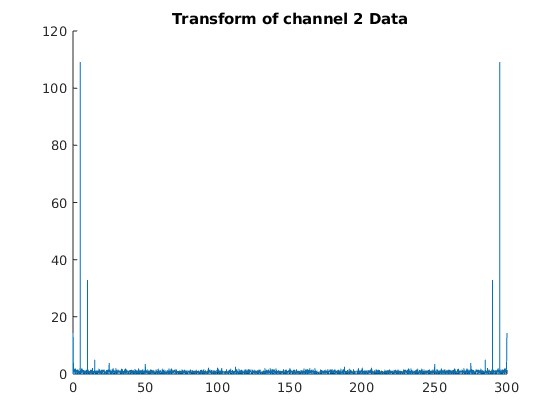
\includegraphics[width=0.85\linewidth]{figures/my_dft.jpg}
      \captionof{figure}{My DFT}
      \label{fig:dft}
    \end{minipage}%
    \hfill
    \begin{minipage}{0.4\textwidth}
      \centering
      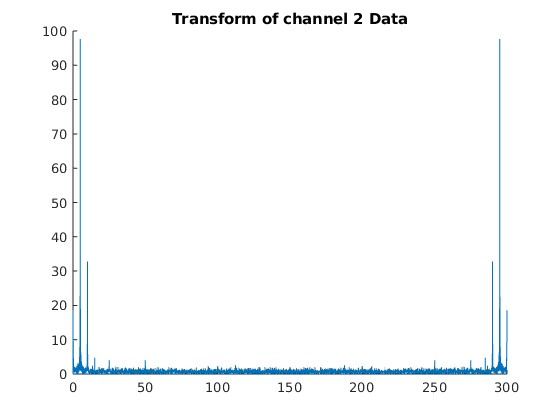
\includegraphics[width=0.85\linewidth]{figures/my_fft.jpg}
      \captionof{figure}{My FFT}
      \label{fig:fft}
    \end{minipage}
    
    % Second row - one image centered
    \begin{minipage}{0.4\textwidth}
      \centering
      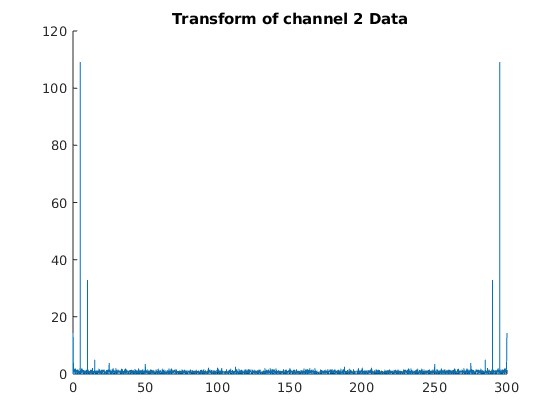
\includegraphics[width=0.85\linewidth]{figures/matlab_fft.jpg}
      \captionof{figure}{MATLAB FFT}
      \label{fig:matlab}
    \end{minipage}
  \end{figure}
\end{frame}



\begin{frame}{Experimental Analysis: Complexity}
    \begin{figure}[h]
        \centering
        \includegraphics[width=0.7\textwidth]{figures/complex.jpg}
        \caption{Execution time versus signal length $N$ for various implementations of FFT}
        \label{fig:complexity}
    \end{figure}
Log-log plots confirm that the FFT scales as \(O(N \log N)\) while the DFT scales as \(O(N^2)\).
\end{frame}

\begin{frame}{Experimental Analysis: Numerical Error}
    \begin{figure}[h]
        \centering
        \includegraphics[width=0.4\textwidth]{figures/recon.jpg}
        \caption{Reconstruction error versus signal length $N$ for various implementations of FFT}
        \label{fig:recon}
    \end{figure}
  \begin{itemize}
    \item The reconstruction error was measured using the RMSE, $\sqrt{\frac{1}{N}\sum_{i=1}^{N}|x_i - \hat{x}_i|^2}$
    \item Although all errors are very low (around \(10^{-12}\)), the custom DFT shows an exponentially growing error with increasing \(N\).
    \item In contrast, both FFT implementations maintained minimal error.
  \end{itemize}
\end{frame}



\section{Windowing}
\subsection{Theory}

% Windowing Theory Slide
\begin{frame}{Why Windowing?}
      \begin{figure}
        \centering
        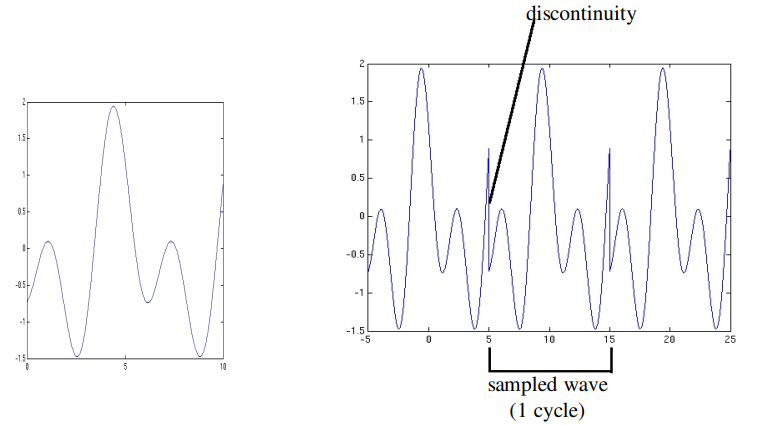
\includegraphics[width=0.6\linewidth]{figures/discontinuous.png}
        \caption{Discontinuities due to truncation}
        \label{fig:1}
        \end{figure}
  \begin{itemize}
    \item  When sampling continuous non-periodic signals, we are only able to sample for a finite time period, resulting in a truncated signal causing discontinuities.
    \item Discontinuities in the time domain become "ripples" in the frequency domain, known as spectral leakage. 
    \end{itemize}
\end{frame}

% Window Functions Slide
\begin{frame}{Why Windowing?}
  \begin{figure}
    \centering
    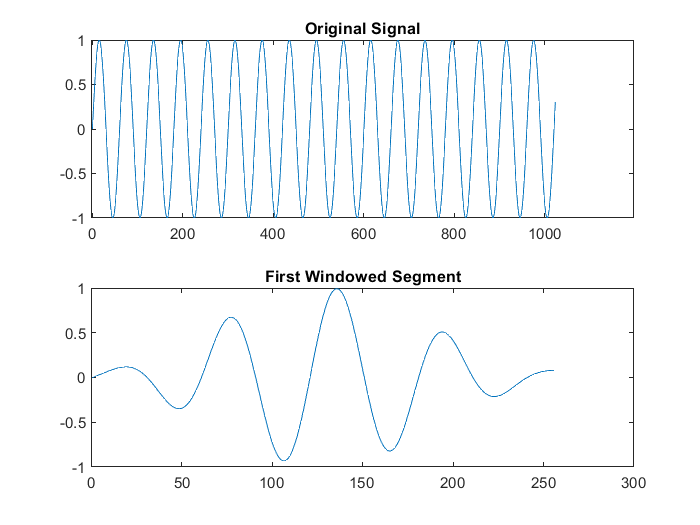
\includegraphics[width=0.6\linewidth]{figures/Hann_window.png}
    \caption{Hann Windowing on sinusoid segment}
    \label{fig:1}
\end{figure}
\begin{itemize}
    \item A “window function” which smooths these edges, reducing unwanted artifacts and improving spectral estimation by reducing the values at the edge of the truncated sample.
    \end{itemize}
\end{frame}

\begin{frame}{Windowing Functions: Hann, Hamming, Blackman-Harris}
  \begin{figure}
    \centering
    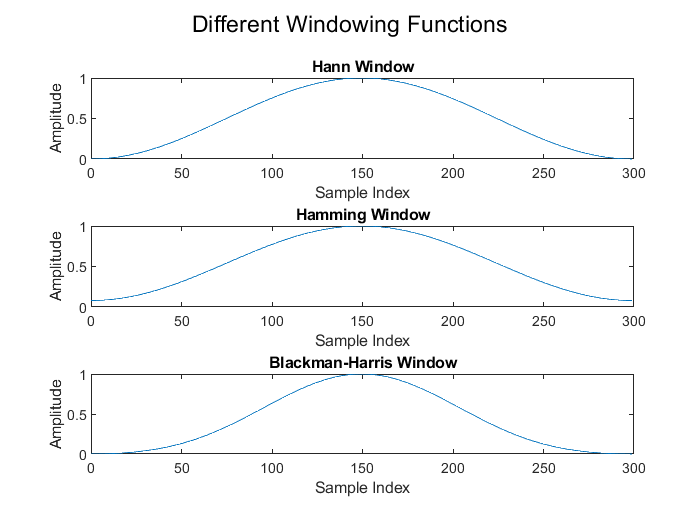
\includegraphics[width=0.6\linewidth]{figures/windowing_functions.png}
    \caption{Discontinuities due to truncation}
    \label{fig:1}
\end{figure}
\end{frame}

% Window Functions Slide
\begin{frame}{Windowing Functions: Hann, Hamming, Blackman-Harris}
  \begin{itemize}
    \item \textbf{Hann Window:} Smoothens the edges using an inverted cosine function.
      \[
0.5*(1-cos(2\pi n / (N - 1)))
  \]
    \item \textbf{Hamming Window:} Similar to Hann but retains a small gap at the edges for a narrower main lobe.
          \[
0.54-0.46cos(2\pi n / (N - 1))
  \]
    \item \textbf{Blackman-Harris Window:} Stronger tapering for better side lobe suppression at the cost of frequency resolution.
                  \[
0.42-0.5cos(2\pi n / (N - 1))+0.8cos(4\pi n / (N - 1)))
  \]
  \end{itemize}
\end{frame}

\begin{frame}{Measurements and Results}
  \begin{itemize}
    \item Implemented the 3 windowing functions in MATLAB.
    \item Applied to a 5Hz sinusoid to observe the impact on peak amplitudes and side lobe suppression.
    \item Results illustrate differences in resolution and leakage for each window.
  \end{itemize}
  \begin{figure}
    \centering
    % First image in its own minipage
    \begin{minipage}{0.48\textwidth}
      \centering
      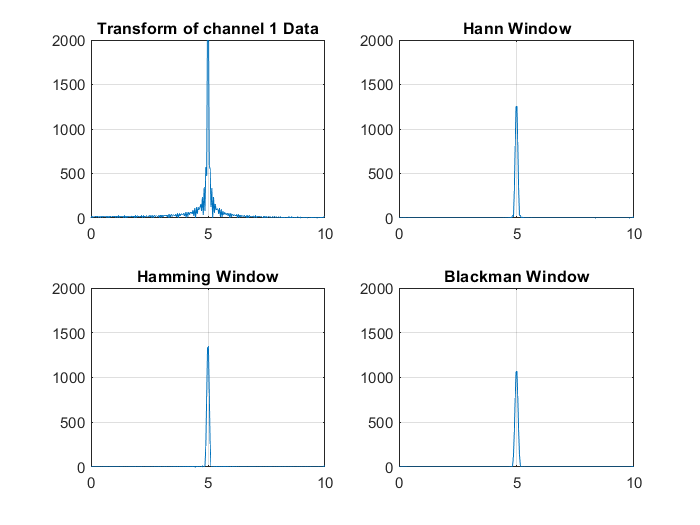
\includegraphics[width=0.9\linewidth]{figures/sin5_window.png}
    \end{minipage}%
    \hfill
    % Second image in its own minipage
    \begin{minipage}{0.48\textwidth}
      \centering
      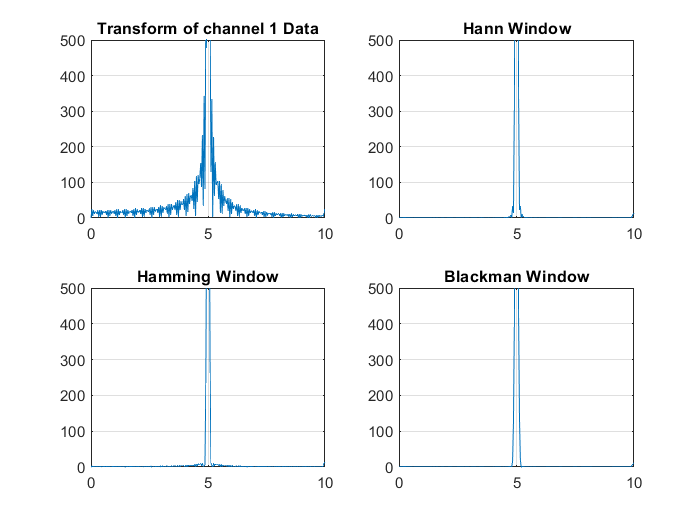
\includegraphics[width=0.9\linewidth]{figures/sin5_window_zoomed.png}
    \end{minipage}
    % A single caption for both images
    \caption{Effect of windowing on amplitude and side lobe suppression.}
  \end{figure}
\end{frame}


\begin{frame}{Measurements and Results}
  \begin{figure}
    \centering
    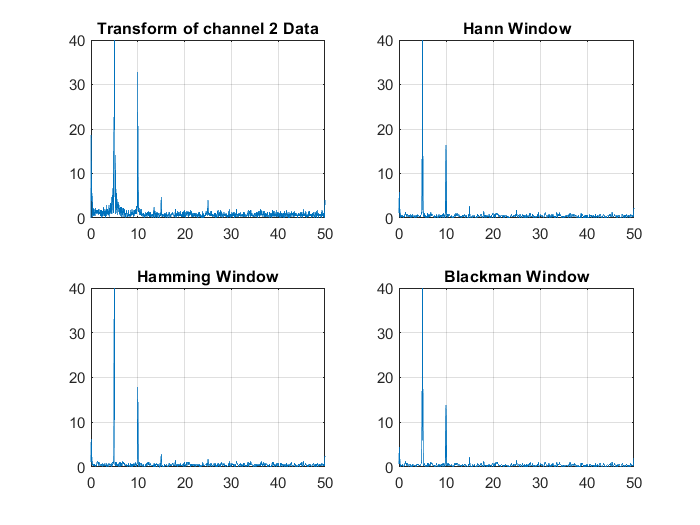
\includegraphics[width=0.6\linewidth]{figures/untitled.png}
    \caption{Windowing function applied to measured ch2 data}
    \label{fig:1}
\end{figure}
\end{frame}


\begin{frame}{Measurements and Results}
  \begin{figure}
    \centering
    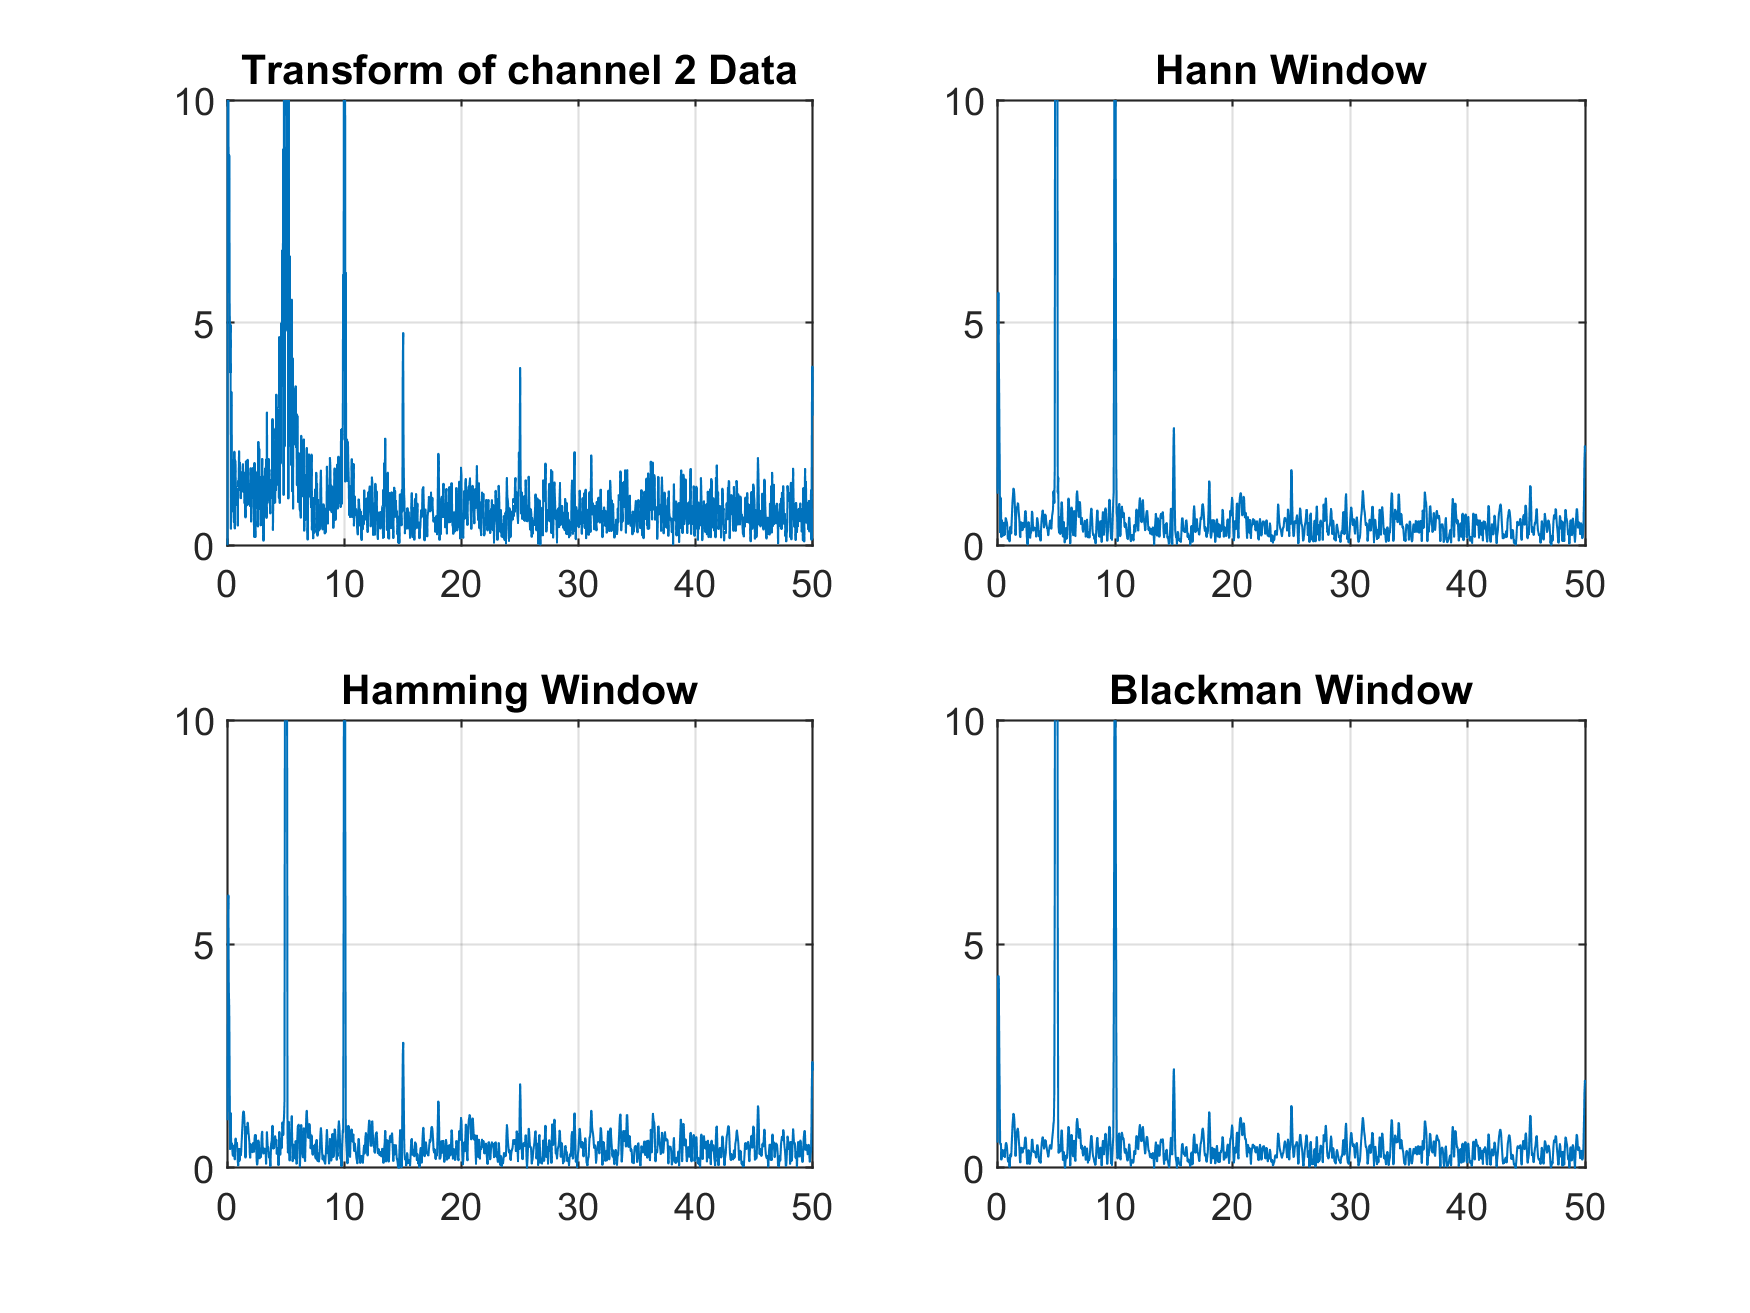
\includegraphics[width=0.6\linewidth]{figures/a4_spectrum_hann.png}
    \caption{Windowing function applied to measured ch2 data}
    \label{fig:1}
\end{figure}
\end{frame}


% Discussion Slide
\begin{frame}{Discussion and Conclusions}
  \begin{itemize}
    \item The choice of a window function depends on the nature of the signal.
    \item \textbf{Hann/Hamming Window:} Suitable for smooth, continuous signals requiring balanced performance.
    \item \textbf{Blackman Window:} Ideal for transient analysis with minimal leakage.
  \end{itemize}
\end{frame}

% Application to Earthquake Data Slide
\begin{frame}{Application to Earthquake Data}
  \begin{itemize}
    \item Earthquakes are characterized by sudden, short-duration energy releases caused by the rupture of faults.
These seismic waves result in strong transients that propagate through the Earth’s crust.
    \item Out of the 3 tested cases, the \textbf{Blackman-Harris Window} may be the most suitable as it offers the best side lobe suppression capabilites. 
    \item Other dynamic functions such as  \textbf{Kaiser Window} with adjustable beta can balance resolution and leakage suppression.
  \end{itemize}
\end{frame}

%%%%%%%%%%%%%%%%%%%%%%%%%%%%%%%%%%%%%%%%%%%%%%%%%%%%%%%%%%%%%%%%%%%%%
\section{Conclusion}

\begin{frame}{Conclusion}
  \begin{itemize}
    \item The direct DFT scales as \(O(N^2)\), which is computationally expensive for large data sets.
    \item The FFT reduces the complexity to \(O(N \log N)\), providing significant performance gains.
    \item Experimental results confirm the expected scaling and show that FFT has superior numerical stability compared to the DFT.
  \end{itemize}
  \begin{itemize}
    \item Selecting the appropriate window is crucial for accurate frequency analysis.
    \item The Hann or Hamming window is recommended for general applications.
    \item Earthquake data benefits from adaptive windows like Kaiser for transient preservation.
  \end{itemize}
\end{frame}

\end{document}



%%%%%%%%%%%%%%%%%%%%%%%%%%%%%%%%%%%%%%%%%%%%%%%%%%%%%%%%%%%%%%%%%%%%%
\end{document}
